%%%%%%%%%%%%%%%%%%%%%%%%%%%%%%%%%%%%%%%%%%%%%%%%%%%%%%%%%%%%%%%%%%%%%%%%%%%%%%%%
%%
%%   BornAgain User Manual
%%
%%   homepage:   http://www.bornagainproject.org
%%
%%   copyright:  Forschungszentrum Jülich GmbH 2015
%%
%%   license:    Creative Commons CC-BY-SA
%%   
%%   authors:    Scientific Computing Group at MLZ Garching
%%               C. Durniak, M. Ganeva, G. Pospelov, W. Van Herck, J. Wuttke
%%
%%%%%%%%%%%%%%%%%%%%%%%%%%%%%%%%%%%%%%%%%%%%%%%%%%%%%%%%%%%%%%%%%%%%%%%%%%%%%%%%


\chapter{DWBA for multilayer systems}  \label{sec:Multilayers}


\index{Multilayer|(}%
\index{Layer structures|see {Multilayer}}

In Sect.~\ref{Sdwba},
we have discussed wave propagation and scattering in 2$+$1 dimensional systems
that are translationally invariant in the horizontal $xy$ plane,
and have a vertical refractive index profile $\nz(z)$.
Here we specialize to layered systems
where $\nz(z)$ is a step function that is constant within one layer.
First, only scalar interactions are considered.
Later, the theory is extended to account for polarization effects.

\Note{\indent By convention,
layers are numbered from top to bottom (see Fig.~\ref{Fdefz}).
The top vacuum (or air) layer (which extends to $z\to+\infty$) has number~0,
\index{Multilayer!numbering}%
\index{Layer!index}%
the substrate (extending to $z\to-\infty$) is layer~$N$.}

All layer interfaces are assumed to be perfectly smooth.
% TODO RESTORE TEMPORARILY REMOVED XREF: 
Support for rough interfaces is already implemented in \BornAgain,
but documentation is adjourned to a later edition of this manual.
% For rough interfaces, see Chapter~\ref{sec:Roughness}.

%%%%%%%%%%%%%%%%%%%%%%%%%%%%%%%%%%%%%%%%%%%%%%%%%%%%%%%%%%%%%%%%%%%%%%%%%%%%%%%%
\section{Scalar case}
%%%%%%%%%%%%%%%%%%%%%%%%%%%%%%%%%%%%%%%%%%%%%%%%%%%%%%%%%%%%%%%%%%%%%%%%%%%%%%%%

%===============================================================================
\subsection{Wave propagation and DWBA matrix element}
%===============================================================================

To compute scattering cross sections in DWBA,
we first need to determine the distorted wavefunctions~$\psi_w(\r)$
for $\r$ inside the sample.
The following derivation holds for the incoming wave ($w=\ti$)
as well as for the back-traced detected wave ($w=\tf$).

\begin{figure}[tb]
\begin{center}
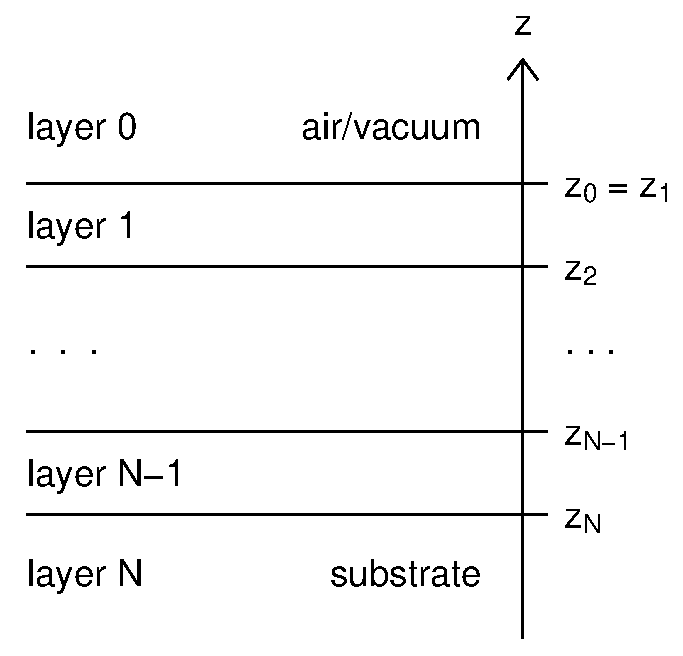
\includegraphics[width=0.4\textwidth]{fig/drawing/multilayer_z_conventions.ps}
\end{center}
\caption{The parameter $z_l$ is the $z$ coordinate of the \E{top} interface
\index{Multilayer!numbering}%
\index{Layer!index}%
\index{Multilayer!coordinates}%
\index{Layer!coordinate}%
of layer~$l$, except for $z_0$ which is the coordinate of the \E{bottom} interface
of the air/vacuum layer~0.}
\label{Fdefz}
\end{figure}

We consider wave propagation in one layer~$\il$
\nomenclature[2l020]{$\il$}{Index of layer in multilayer sample}%
with constant average refractive index $\nz(z)=\nzj$.
A vacuum plane wave, impinging on a layered structure,
is at each interface partly reflected, partly refracted,
so that the wavefunction inside a material layer
has an upward and a downward propagating component,
as per~(\ref{Epsipm}).
Each component is a plane wave,
with a wavevector
\begin{equation}\label{Ekpmwj3}
  \k^\pm_{w\il}= \k_{\parallel w} \pm k_{\perp w\il}\v{\hat z}.
\end{equation}
\nomenclature[2z060]{$\v{\hat z}$}{Unit vector along the sample normal}%
\nomenclature[2k043 2w010 2l010 \pm]{$\k^\pm_{w\il}$}{wavevector of the plane wave $\psi^\pm_{w\il}(\r)$}%
As explained in connection with~(\ref{Ekpar}),
the in-plane wavevector $\k_{\parallel w}$ remains constant
across layer interfaces.
The vertical wavenumber is obtained from (\ref{Ewavez}),
\begin{equation}\label{Ekperpwj}
  k_{\perp w\il} = \sqrt{K^2 \nzj - k_{\parallel w}^2}.
\end{equation}
We factorize the corresponding wavefunctions as
\begin{equation}
  \psi^\pm_{w\il}(\r)=\e^{i\k_{\parallel w}\r_\parallel}\phi^\pm_{w\il}(z),
\end{equation}
with vertical propagation described by a one-dimensional wavefunction
\begin{equation}\label{Ephizwj}
  \phi^\pm_{w\il}(z)=A^\pm_{w\il}\e^{\pm ik_{\perp w\il}(z-z_\il)}.
\end{equation}
\nomenclature[2a123 2w010 2l010 \pm]{$A^\pm_{w\il}$}{Amplitude of the plane wave $\phi^\pm_{w\il}(\r)$}%
For later convenience,
the phase factor in (\ref{Ephizwj}) includes an offset~$z_\il$
as defined in Fig.~\ref{Fdefz}.
\nomenclature[2z020 2l010]{$z_l$}{Vertical coordinate at the top of layer~$l$ (at the bottom for $l=0$)}%
\index{Multilayer!coordinates}%
\index{Layer!coordinate}%
The amplitudes $A$ are often written with distinct letters
T and~R to designate the transmitted or reflected beam,
\begin{equation}
  T_{w\il} \coloneqq  A^-_{w\il},\quad
  R_{w\il} \coloneqq  A^+_{w\il}.
\end{equation}
\nomenclature[2t126 2w020 2l020 0]{$T_{w\il}$}{Partial amplitude of $\psi_w(\r)$
  in layer $\il$ in downward (transmission) direction, also denoted $A^-_{w\il}$}%
\nomenclature[2r126 2w020 2l020 0]{$R_{w\il}$}{Partial amplitude of $\psi_w(\r)$
  in layer $\il$ in upward (reflection) direction, also denoted $A^+_{w\il}$}%
They need to be computed recursively,
as described in the following subsection~\ref{Sacrolay}.

In the absence of absorption,
wavevectors are real
so that we can describe the beam in terms of a glancing angle
\begin{equation}\label{Edef_alpha}
  \alpha_{w\il}\coloneqq \arctan(k_{\perp w\il}/k_{\parallel w}).  
\end{equation}
Equivalently,
\begin{equation}
  k_{\parallel w}=K n_\il \cos\alpha_{w\il}. 
\end{equation}
Since $k_{\parallel w}$ is constant across layers,
we have
\begin{equation}\label{ESnell}
  n_\il \cos\alpha_{w\il} = \text{the same for all }\il,
\end{equation}
which is Snell's refraction law.
\index{Refraction!Snell's law}
\index{Snell's law}

Since the $\psi^\pm_{w\il}$ are plane waves within layer~$\il$,
we can at once write down the DWBA transition matrix element~(\ref{Edwba})
\index{Distorted-wave Born approximation!multilayer}%
\begin{equation}\label{Edwba_ml0}
  \bra \psi_\ti|\chi|\psi_\tf\ket
  = \sum_{\il} \sum_{\pm_\ti} \sum_{\pm_\tf}
    A^{\pm *}_{\ti \il} A^\pm_{\tf \il} 
     \chi_\il(\k^\pm_{\tf \il}-\k^\pm_{\ti \il}),
\end{equation}
where
\begin{equation}\label{Echij}
  \chi_\il(\v{q})
  \coloneqq  \int_{z_\il}^{z_{\il-1}}\!\d z \int\!\d^2r_\parallel\, \e^{i\v{q}\,\r}\chi(\r)
\end{equation}
\nomenclature[1χ032 2l010 2q040]{$\chi_\il(\v{q})$}{Fourier transform of the perturbation potential $\chi(\r)$, evaluated in one sample layer}%
is the Fourier transform
of the perturbative potential~(\ref{EChiGraded}),
restricted to one layer.

To alleviate later calculations,
we now number the four DWBA terms from 1 to 4,
and define the corresponding wavenumbers and amplitude factors and as
\begin{equation}
  \begin{array}{l@{\hspace{2em}}l}
    \q^1 \coloneqq  \k^-_\tf - \k^-_\ti,& C^1 \coloneqq  A^{-*}_\ti A^-_\tf, \\[.6ex]
    \q^2 \coloneqq  \k^-_\tf - \k^+_\ti,& C^2 \coloneqq  A^{-*}_\ti A^+_\tf, \\[.6ex]
    \q^3 \coloneqq  \k^+_\tf - \k^-_\ti,& C^3 \coloneqq  A^{+*}_\ti A^-_\tf, \\[.6ex]
    \q^4 \coloneqq  \k^+_\tf - \k^+_\ti,& C^4 \coloneqq  A^{+*}_\ti A^+_\tf.
  \end{array}
\end{equation}
Accordingly, we can write (\ref{Edwba_ml0}) as
\Emph{
\begin{equation}\label{Edwba_ml}
  \bra \psi_\ti|\chi|\psi_\tf\ket
  = \sum_{\il} \sum_{u} C^u_\il \chi_\il(\q_\il^u).
\end{equation}
\vspace*{-5pt}}
From~(\ref{Ekpmwj3}) we see that all four wavevectors $\q^u$
have the same horizontal component,
\begin{equation}\label{Eqpp}
  \q^u = \q_\parallel + q^u_\perp \v{\hat z}
\end{equation}
whence the vertical components
\begin{equation}
    \begin{array}{l}
  q^1_\perp = +k_{\tf\perp  } -k_{\ti\perp},\\[.6ex]
  q^2_\perp = +k_{\tf\perp  } +k_{\ti\perp},\\[.6ex]
  q^3_\perp = -k_{\tf\perp  } -k_{\ti\perp},\\[.6ex]
  q^4_\perp = -k_{\tf\perp  } +k_{\ti\perp}.
    \end{array}
\end{equation}

%-------------------------------------------------------------------------------
\subsection{Wave propagation across layers}\label{Sacrolay}
%-------------------------------------------------------------------------------

\index{Fresnel coefficients}%
\index{Transmission|see {Fresnel coefficients}}%
\index{Reflection|seealso {Fresnel coefficients}}%

The plane-wave amplitudes $A^\pm_{w\il}$ need to be computed recursively
from layer to layer.
Since these computations are identical for incident and final waves,
we omit the subscript~$w$ in the remainder of this section.
At layer interfaces, the optical potential changes discontinuously.
From elementary quantum mechanics we know that
piecewise solutions of the Schrödinger equations must be connected
such that the wavefunction $\phi(\r)$ and its first derivative
$\Nabla\phi(\r)$ evolve continuously.

To deal with the coordinate offsets introduced in (\ref{Ephizwj}),
we introduce the function
\begin{equation}
  d_\il\coloneqq z_{\il}-z_{\il+1},
\end{equation}
which is the thickness of layer~$\il$,
except for $\il=0$,
where the special definition of $z_0$ (Fig.~\ref{Fdefz}) implies $d_0=0$.
We consider the interface between layers $\il$ and $\il+1$,
with~$\il=0,\ldots,N-1$.
This interface has the vertical coordinate $z_{\il+1}=z_l-d_l$.
Accordingly, the continuity conditions at the interface are
\begin{equation}\label{Econtcond}
  \begin{array}{lcl}
  \hphantom{\partial_z}\phi_{\il+1}(z_{\il+1}) &=& \hphantom{\partial_z}\phi_{\il}(z_{\il}-d_{\il}),\\
            \partial_z \phi_{\il+1}(z_{\il+1}) &=&           \partial_z \phi_{\il}(z_{\il}-d_{\il}).
  \end{array}
\end{equation}
We abbreviate
\begin{equation}
  f_\il \coloneqq  k_{\perp \il}/K = \sqrt{\nzj-(k_\parallel/K)^2}
\end{equation}
and
\begin{equation}
   \delta_\il \coloneqq  \e^{iKf_\il d_\il}.
\end{equation}
For the plane waves (\ref{Ephizwj}),
the continuity conditions~(\ref{Econtcond}) take the form
\begin{equation}\label{Econt2}
  \begin{array}{@{}l@{}lcl@{}l}
  +A^-_{\il+1} &+A^+_{\il+1}
  &=&
  +A^-_{\il}\delta_{\il} &+A^+_{\il}\delta_{\il}^*,
  \\
  -A^-_{\il+1} f_{\il+1}  &+A^+_{\il+1} f_{\il+1}
  &=&
  -A^-_{\il}\delta_{\il} f_{\il} &+A^+_{\il}\delta_{\il}^* f_{\il}.
  \end{array}
\end{equation}
After some lines of linear algebra,
we can rewrite this equation system as
\begin{equation}\label{EcMc}
  \left( \begin{array}{c}A^-_{\il}\\ A^+_{\il}\end{array} \right)
  = M_{\il} \left( \begin{array}{c}A^-_{\il+1}\\A^+_{\il+1}\end{array} \right)
\end{equation}
with the transfer matrix
\begin{equation}
  M_\il
   \coloneqq
   \left(\begin{array}{cc}
       \delta_\il^*&0\\
       0 & \delta_\il
   \end{array}\right)
   \frac{1}{2f_{\il}}
   \left(\begin{array}{cc}
       (f_{\il}+f_{\il+1})&(f_{\il}-f_{\il+1})\\
       (f_{\il}-f_{\il+1})&(f_{\il}+f_{\il+1})
   \end{array}\right).
\end{equation}

In our scattering setup,
plane-wave amplitudes are subject to two boundary conditions:
In the top layer, $A^-_{0}=1$ is given by the
incident or back-traced final plane wave.
In the substrate, $A^+_{N}=0$ because there is no radiation
coming from $z\to-\infty$.
This leaves us with two unkown amplitudes,
the overall coefficients of transmission~$A^-_N$ and reflection~$A^+_0$.
These two unknowns are  connected by a system of two linear equations,
\begin{equation}
  \left( \begin{array}{c}1\\ A^+_0\end{array} \right)
  = M_0 \cdots M_{N-1} \left( \begin{array}{c}A^-_N\\0\end{array} \right).
\end{equation}
While it is possible in principle
to solve this as a matrix equation,
the actual implementation in \BornAgain\ 
%\footnote{SpectralMatrix.cpp: SpectralMatrix::execute()}
starts with a unit vector in the substrate,
and then carries out the propagation step (\ref{EcMc})
interface by interface,
yielding unnormalized amplitudes
\begin{equation}\label{EAtildel}
  \left( \begin{array}{c}\tilde A^-_{\il}\\ \tilde A^+_{\il}\end{array} \right)
  \coloneqq M_{\il}\cdots M_{N-1} \left( \begin{array}{c}1\\0\end{array} \right).
\end{equation}
When the top layer is reached,
the obtained values are renormalized
so that the boundary condition $A^-_{0}=1$ be satisfied,
\begin{equation}
  A^\pm_{\il} = \frac{\tilde A^\pm_l}{\tilde A^-_0}.
\end{equation}

At this point,
it may be an interesting exercise to make
 a connection with a well known textbook result.
Consider a system
with a single interface between two semi-infinite media.
A straightforward computation will show
that the transmission and reflection probabilities
determined as above
agree with Fresnel's result for $s$-polarized light,\footnote
{See any optics textbook, e.g.\ Born~\&~Wolf \cite[ch.~1.5.2]{BoWo99}
  or Hecht \cite[ch.~4.6.2]{Hec02}.}
\begin{equation}
  \left| A^-_N\right|^2
  = \left| \frac{2f_0}{f_0+f_1}\right|^2,
  \quad
  \left| A^+_0\right|^2
  = \left|\frac{f_0-f_1}{f_0+f_1}\right|^2.
\end{equation}

The above algorithm fails if $f_l\to0$
because $M_l$ becomes singular.
A layer with $f_l=0$ only sustains horizontal wave propagation;
radiation from below or above is totally reflected at its boundaries.
In \BornAgain,
such total reflection is imposed if $|f_l|$ falls below a very small value
(currently $10^{-20}$).
However, this has hardly any practical importance
because except in vacuum the index of refraction always
as an absorptive component that prevents $f_l$ from becoming zero.


%-------------------------------------------------------------------------------
\subsection{Damped waves in absorbing media or under total reflection}
  \label{Smulayabs}
%-------------------------------------------------------------------------------

In Sect.~\ref{Sabsorption},
we have chosen the horizontal wavevector $\k_{\parallel}$
to be always real and constant.
In contrast, the vertical wavenumber $k_{\perp \il}$,
given by (\ref{Ekperpwj}),
can become imaginary or complex.
If $\overline{n_\il^2}$ is real and smaller than~$n_0^2\cos^2\alpha_0$,
then Snell's law of refraction (\ref{ESnell}) cannot be fulfilled,
and the radicand in (\ref{Ekperpwj}) becomes negative
so that $k_{\perp \il}$ becomes pure imaginary.
\index{Wavevector!complex}%
If the layer is absorbing,
described by a positive imaginary part of $\overline{n_\il^2}$,
then the radicand in (\ref{Ekperpwj}) becomes complex,
and the wavenumber $k_{\perp \il}$ as well.
For complex $k_{\perp \il}$,
the theory developed above remains applicable,
except that the geometric interpretation of the wavevectors $\k_\pm$
in Eqs.~(\ref{Edef_alpha}--\ref{ESnell}) is untenable.

Writing
\begin{equation}
  k_\perp = k_\perp' + i k_\perp''
\end{equation}
for a decomposition into a real and an imaginary part,
we find an exponential decay of the plane wave amplitudes
\begin{equation}\label{Ephidamp}
  \left|\phi^\pm_\il(z)\right|
  = \e^{\mp k_{\perp \il}'' z}
\end{equation}
along their propagation direction~$\pm z$.
With an analogous decomposition
of the three-dimensional wavevector (\ref{Ekpmwj3}),
we obtain for the flux, defined as in~(\ref{EdefJ}),
\begin{equation}
  \v{J}_\il(\r) = \k' \e^{-2k_{\perp \il}z}.
\end{equation}
In the special case of a pure imaginary~$k_{\perp \il}$,
the flux direction is $\k'=\k_\parallel$.
Then $\psi_\il(\r)$ is an \E{evanescent wave},
\index{Evanescent wave}%
travelling horizontally.
Since a stationary evanescent wave implies that there is
no vertical energy transport,
all incoming radiation undergoes \E{total reflection}.
\index{Total reflection}%

In the generic case of a complex~$k_{\perp \il}$,
the flux has a vertical component.
Accordingly, the total reflection is not perfect.
Some intensity is dissipated in layer $\il$.
\index{Dissipation}%
And if layer $\il<N$ is not too thick,
then some radiation intensity also tunnels into the adjacent layer $\il+1$.
\index{Tunneling}%

%%%%%%%%%%%%%%%%%%%%%%%%%%%%%%%%%%%%%%%%%%%%%%%%%%%%%%%%%%%%%%%%%%%%%%%%%%%%%%%%
% \newpage % TEMPORARY
%\section{Reflection with polarization-dependent interactions}\label{s:pol}
%%%%%%%%%%%%%%%%%%%%%%%%%%%%%%%%%%%%%%%%%%%%%%%%%%%%%%%%%%%%%%%%%%%%%%%%%%%%%%%%

%\MissingSection
% %\Work{\indent To be reinserted once
% the chapter on polarized waves propagation is written.}
\iffalse

%\cite{Deak_ppt, PhysRevB.76.224420, Deak2001113, PhysRevB.53.6158}.
%\cite{RevModPhys.23.287}

%-------------------------------------------------------------------------------
\subsection{Wave equation and propagation within one layer}
%-------------------------------------------------------------------------------

To allow for polarization-dependent interactions,
we replace the squared index of refraction $n^2$
by $1+\uu\chi$, where $\uu\chi$ is a $2\times 2$ susceptibility matrix.
The wave equation (\ref{Escalar_wave}) for layer~$\il$ becomes
\begin{equation}\label{Ewaveqp}  
(\Delta +K^2 +K^2 \uu\chi_\il) \u\psi(\r)= 0,
\end{equation}
where $\u\psi(\r)$ is a two-component spinor wavefunction,
with components $\psi_\UP(\r)$ and~$\psi_\DN(\r)$.
At interfaces between layers,
both spinor components of $\u\psi(\r)$ and $\Nabla\u\psi(\r)$
must evolve continuously.

The reasons for the factorization (\ref{Ewave3}) still apply,
and so we can write
\begin{equation}\label{Ewave3p}
\u\psi(\r) = \u\psi(z) \e^{i \k_\parallel\r_\parallel}.
\end{equation}
As before, $\k_\parallel$ is constant across layers.
The wave equation~(\ref{Ewaveqp}) reduces to 
\begin{equation}\label{Ewavezp}
\left(\partial_z^2 + K^2 + K^2\uu\chi_\il - k_\parallel^2 \right) \u\psi(z) = 0.
\end{equation}
We abbreviate
\begin{equation}
  \uu H_\il \coloneqq  K^2(1+\uu\chi_\il)-k_\parallel^2
\end{equation}
so that the wave equation becomes simply
\begin{equation}\label{Ewaveqp2}
  \left(\partial_z^2 + \uu H_\il\right) \u\psi(z) = 0.
\end{equation}
The solution is
\begin{equation}\label{Epsizp}
  \u\psi_\il(z)
  = \sum_{k=1}^2 \u x_{\il k}\left(\alpha_{\il k}\e^{i p_{\il k}(z-z_k)}
                            + \beta_{\il k}\e^{-i p_{\il k}(z-z_k)}\right),
\end{equation}
where the $\u x_{\il k}$ are eigenvectors of $\uu H_\il$
with eigenvalues $p_{\il k}^2$:
\begin{equation}
  \left( -p_{\il k}^2 + \uu H_\il \right) \u x_{\il k} = 0
   \;\text{ for }\;\il=1,2.
\end{equation}
In a reproducible algorithm,
the eigenvectors $\u x_{\il k}$ must be chosen according to some arbitrary
normalization rule,
for instance
\begin{equation}
  |\u x_{\il k}|=1,\quad x_{i\il\UP} \text{ real and nonnegative}.
\end{equation}
Similarly,
a rule is needed how to handle the case of one degenerate eigenvalue,
which includes in particular the case of scalar interactions.


%-------------------------------------------------------------------------------
\subsection{Wave propagation across layers}
%-------------------------------------------------------------------------------

Generalizing (\ref{Evecc}),
we introduce the coefficient vector
\begin{equation}
  c_\il \coloneqq  {(\alpha_{\il1}, \alpha_{\il2}, \beta_{\il1}, \beta_{\il2})}^\text{T}.
\end{equation}
To match solutions for neighboring layers,
continuity is requested for both spinorial components
of $\u\psi$ and $\Nabla\u\psi$.
As before (\ref{EFcFDc}), we have at the bottom of layer~$\il$
\begin{equation}\label{EFcFDcp}
  F_\il c_\il = F_{\il+1} D_{\il+1} c_{\il+1},
\end{equation}
where the matrices are now
\begin{equation}
  F_\il \coloneqq  \left(\begin{array}{cccc}
    x_{i1\UP}      &x_{i2\UP}     &x_{i1\UP}       &x_{i2\UP}       \\
    x_{i1\DN}      &x_{i2\DN}     &x_{i1\DN}       &x_{i2\DN}       \\
    x_{i1\UP}p_{\il1}&x_{i2\UP}p_{\il2}&-x_{i1\UP}p_{\il1}&-x_{i2\UP}p_{\il2}\\
    x_{i1\DN}p_{\il1}&x_{i2\DN}p_{\il2}&-x_{i1\DN}p_{\il1}&-x_{i2\DN}p_{\il2}
  \end{array}\right)
\end{equation}
and
\begin{equation}
  D_\il \coloneqq  \text{diag}(\delta_{\il1}, \delta_{\il2}, \delta_{\il1}^*, \delta_{\il2}^*)
\end{equation}
with the phase factor
\begin{equation}
   \delta_{\il k} \coloneqq  \e^{ip_{\il k}d_k}.
\end{equation}
Note that matrix $F_\il$ has the block form
\begin{equation}
  F_\il
  =\left(\begin{array}{ll}\uu x_\il&\hphantom{-}\uu x_\il\\[1ex]
    \uu x_\il\; \uu P_\il&-\uu x_\il\; \uu P_\il\end{array}\right)
    = \uu x_\il \cdot
    \left(\begin{array}{cc}\uu 1&\uu 1\\[1ex]
    \uu P_\il&-\uu P_\il\end{array}\right),
\end{equation}
with
\begin{equation}
  \uu x_\il \coloneqq 
  \left(\u x_{\il1}, \u x_{\il2}\right),
  \quad
  \uu P_\il \coloneqq 
  \text{diag}\left(p_{\il1},p_{\il2}\right).
\end{equation}
This facilitates the computation of the inverse
\begin{equation}
  F_\il^{-1}
    = \frac{1}{2}
    \left(\begin{array}{cc}\uu 1&\hphantom{-}\uu P_\il^{-1}\\[1.2ex]
      \uu 1 &-\uu P_\il^{-1}\end{array}\right)
      \cdot\uu x_\il^{-1},
\end{equation}
which is needed for the transfer matrix $M_\il$,
defined as in (\ref{Edef_M}).
With the new meaning of $c_\il$ and $M_\il$,
the recursion (\ref{EcMc}) and the explicit solution~(\ref{Eci})
hold as derived above.
To resolve~(\ref{Eci}) for the reflected amplitudes $\alpha_{0\il}$
as function of the incident amplitudes $\beta_{0\il}$,
we choose the notations
\begin{equation}
  \u\alpha_\il
  \coloneqq \left(\begin{array}{c}\alpha_{\il1}\\\alpha_{\il2}\end{array}\right),\quad
  \u\beta_\il
  \coloneqq \left(\begin{array}{c}\beta_{\il1}\\\beta_{\il2}\end{array}\right),\quad
  M\coloneqq M_1 ... M_N % TODO restore \cdots
  \eqqcolon \left(\begin{array}{cc}\uu m_{11}&\uu m_{12}\\
                           \uu m_{21}&\uu m_{22}\end{array}\right),
\end{equation}
where the $\uu m_{\il k}$ are $2\times2$ matrices.
Eq.~(\ref{Eci}) then takes the form
\begin{equation}
  \left(\begin{array}{c}\u\alpha_{0}\\\u\beta_{0}\end{array}\right)
  = 
  \left(\begin{array}{cc}\uu m_{11}&\uu m_{12}\\
    \uu m_{21}&\uu m_{22}\end{array}\right)
  \left(\begin{array}{c}\u{0}\\\u\beta_{N}\end{array}\right),
\end{equation}
which immediately yields
\begin{equation}
  \u\alpha_0 = \uu m_{12}\,\uu m_{22}^{-1}\,\u\beta_0.
\end{equation}

\fi

\index{Multilayer|)}%
